% Created: Enze Chen, June 2025
%
% Chapter 11 of the MSE 142 coursereader. This chapter introduces ideas in quantum computing as an advanced extension of the course themes.

% Uncomment the following three lines and last line to individually compile this chapter
\documentclass[12pt, english]{book}
\usepackage{142crstyle}
\begin{document}

\chapter[Quantum computing]{Work in Progress:\\Quantum Computing} \label{ch:computing}
%{ \doublespacing 
As an advanced topic, we'll discuss the advantages of quantum computing.


For more information, see this article: https://dl.acm.org/doi/10.1145/367701.367709
or this book: https://doi.org/10.1093/oso/9780192857972.001.0001


%%%%%%%%%%%%%%%%%%%%%%%%%%%%%%%%%%%%%%%%%%%%%%%%%%%%%%%%%%%%%%%%%%%%%%%%%%%%%%%%

\section{Before you begin}

This chapter builds on the following concepts, some of which we've already discussed in class, others you will likely have encountered elsewhere.
We include links to resources that may aid your review, as mastery of these concepts will allow you to get the most out of this chapter.

\begin{itemize}
	\item foo 
	\item bar 
	\item Prerequisite self-check quiz 
\end{itemize}


%%%%%%%%%%%%%%%%%%%%%%%%%%%%%%%%%%%%%%%%%%%%%%%%%%%%%%%%%%%%%%%%%%%%%%%%%%%%%%%%


\section{Introduction to formalisms}

Imagine a general two-level system, which could represent spin states or a light-activated system, that we will represent as $\ket{0}$ and $\ket{1}$.
We could write them in a different way, in vector notation, as follows:

\begin{equation*}
	\ket{0} = \begin{pmatrix} 1 \\ 0 \end{pmatrix}, \qquad \ket{1} = \begin{pmatrix} 0 \\ 1 \end{pmatrix} 
\end{equation*}

These are the basis states, similar to our discussion of polarization in Chapter 1.
To help visualize their linear independence, we could even draw them being orthogonally arranged on the page (e.g., aligned with the $x$- and $y$-axis, respectively), but in no sense do these states have any real-space directions!

Given the basis states $\ket{0}$ and $\ket{1}$, we can write the general superposition state as 

\begin{equation*}
	\ket{\psi} = \alpha \ket{0} + \beta \ket{1},
\end{equation*}

where $\alpha$ and $\beta$ are coefficients such that $\abs{\alpha}^2 + \abs{\beta}^2 = 1$.
An example superposition state is $\ket{\psi} = \dfrac{1}{\sqrt{2}} \left( \ket{0} + \ket{1} \right)$, where we note that $\abs{\psi} = 1$.

Now imagine we have a system with two qubits.
We can represent the states of this system as $\ket{q_1 q_2}$, where $q_i$ represents the state of the $i$th qubit.
For example, $\ket{00}$ would represent qubits 1 and 2 both in the \texttt{0} state.
Continuing in the framework of the vector notation from before, we can express all four possible states as

\begin{equation*}
	\ket{00} = \begin{pmatrix} 1 \\ 0 \\ 0 \\ 0 \end{pmatrix}, \qquad 
	\ket{01} = \begin{pmatrix} 0 \\ 1 \\ 0 \\ 0 \end{pmatrix}, \qquad 
	\ket{10} = \begin{pmatrix} 0 \\ 0 \\ 1 \\ 0 \end{pmatrix}, \qquad 
	\ket{11} = \begin{pmatrix} 0 \\ 0 \\ 0 \\ 1 \end{pmatrix}
\end{equation*}

where we have four unit vectors that comprise an orthogonal basis set in a 4-dimensional space.
Thus we can encode using binary notation the equal-weighted two-qubit state and express it as

\begin{equation*}
	\ket{\psi} = \frac{1}{2} \left( \ket{00} + \ket{01} + \ket{10} + \ket{11} \right) = \frac{1}{2} \left( \ket{0} + \ket{1} + \ket{2} + \ket{3} \right)
\end{equation*}

More generally, we could say that $\ket{\psi} = \dfrac{1}{\sqrt{2^n}} \displaystyle\sum_{x=0}^{2^n-1} \alpha_x \ket{x}$.

If we continue in this vein, we will find that for $n$ qubits there are $2^n$ possibilities!
Encodes $2^n$ numbers. 
How large is this? 
Well, for $n \sim 270$, $2^n$ would be larger than the number of atoms in the universe!\footnote{Which current estimates place at $10^{80}$, see the \href{https://en.wikipedia.org/wiki/Eddington_number}{Eddington number}.}
It would be quite remarkable to store all this information in just 200 atoms!
Even a more modest number like $n = 100$ would give us $10^{30}$ bits, which is equal to $\sim 10^{29}$ or 1 billion zettabytes. 
The global datasphere is only 150 zettabytes (but quickly growing)!
If we could implement a function on this superposition state, then the function would be evaluated on all inputs in parallel.

\begin{equation*}
	\ket{\psi} \rightarrow \boxed{f} \rightarrow \dfrac{1}{\sqrt{2^n}} \sum_{x=0}^{2^n-1} \alpha_x \ket{x}
\end{equation*}

where $f$ is a quantum gate.
The assumption here is that we have a linear operator. 
Actually: operators are unitary and reversible.

But there's a problem: If we make a measurement, we get a single number!
The superposition state collapses, as we saw earlier in the course.
There is no obvious way to sample coefficients.

Perhaps... we can try to be clever and make many copies and then measure many times to sample?
Unfortunately not---the quantum no-cloning theorem!

\textbf{Put the definition box for no-cloning theorem here}

We'll sketch the idea for this theorem below.
Suppose there is an operator $U$ that is linear (and unitary) that can clone an arbitrary state $\ket{\psi} = \alpha \ket{0} + \beta \ket{1}$.
We would have the configuration picture in \autoref{fig:no-clone-1}.

\begin{figure}[!ht]
	\centering
	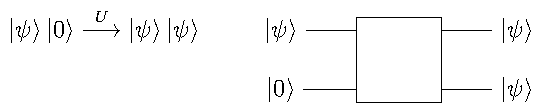
\includegraphics[width=0.6\linewidth]{no-clone-1.pdf}
	\caption{Caption}
	\label{fig:no-clone-1}
\end{figure}

But 
\begin{align*}
	\ket{\psi} \ket{\psi} &= \left( \alpha \ket{0} + \beta \ket{1} \right) \otimes \left( \alpha \ket{0} + \beta \ket{1} \right) \\
	&= \alpha^2 \ket{00} + \alpha \beta \ket{01} + \beta \alpha \ket{10} + \beta^2 \ket{11}
\end{align*}

But on the other hand, 
\begin{align*}
	U \left( \ket{\psi} \ket{0} \right) &= U \left( \alpha \ket{0} + \beta \ket{1} \right) \ket{0} \\ 
	&= \alpha U \ket{00} + \beta U \ket{1} \ket{0} \\
	&= \alpha \ket{00} + \beta \ket{11}
\end{align*}

and the cross terms are missing.
This means cloning is impossible! 

For a different proof, suppose there exists a unitary cloning operator $U$.
This would satisfy 
\[ \ket{\psi 0} \stackrel{U}{\rightarrow} \ket{\psi \psi}\ \text{for all}\ \psi \]

Thus, $U \ket{00} = \ket{00}$ and $U\ket{10} = \ket{11}$.
If we apply this to $H \ket{0} = \frac{1}{\sqrt{2}} \left( \ket{0} + \ket{1} \right)$, we get $U \frac{1}{\sqrt{2}} \left( \ket{0} + \ket{1} \right) \ket{0} = \frac{1}{\sqrt{2}} \left( \ket{00} + \ket{11} \right)$ by linearity.

But this is not successfully cloned, since it should equal
\[ \frac{1}{2} \left( \ket{0} + \ket{1} \right) \left( \ket{0} + \ket{1} \right) = \frac{1}{2} \left( \ket{00} + \ket{01} + \ket{10} + \ket{11} \right) \]
Therefore, $U$ does not exist.


\section{Allowed operators}

So what kind of operators are allowed?
For quantum logic gates, we have
\begin{itemize}
	\item The first example is $H$ that satisfies $H \ket{\psi} = i \hbar \pdv{t} \ket{\psi}$ which gives time evolution.
	
	\item \texttt{NOT} (or $X$ gate), which maps $\ket{0} \rightarrow \ket{1}$ and $\ket{1} \rightarrow \ket{0}$.
	The matrix representation of this is $\begin{pmatrix} 0 & 1 \\ 1 & 0 \end{pmatrix}$, so $\begin{pmatrix} 0 & 1 \\ 1 & 0 \end{pmatrix} \begin{pmatrix} 1 \\ 0 \end{pmatrix} = \begin{pmatrix} 0 \\ 1 \end{pmatrix}$.
	
	\item $Z$ gate, which maps $\ket{0} \rightarrow \ket{0}$ but $\ket{1} \rightarrow -\ket{1}$.
	Written out more fully, $Z \left( \alpha \ket{0} + \beta \ket{1} \right) \rightarrow \alpha \ket{0} - \beta \ket{1}$, which induces a phase flip. 
	The matrix representation of this gate is $\begin{pmatrix} 1 & 0 \\ 0 & -1 \end{pmatrix}$.
\end{itemize}


\section{Bloch sphere}

Another way to visualize the qubit state is on a construct called the \textbf{Bloch sphere} (\autoref{fig:bloch-sphere}), which has $\ket{0}$ and $\ket{1}$ on the north and south pole, respectively, and all possible qubit states represented on the surface of the sphere.
Note that classical bits are restricted to exactly $\ket{0}$ or $\ket{1}$, but quantum allows everything in between.

\begin{figure}[!ht]
	\centering
	\subfloat[]{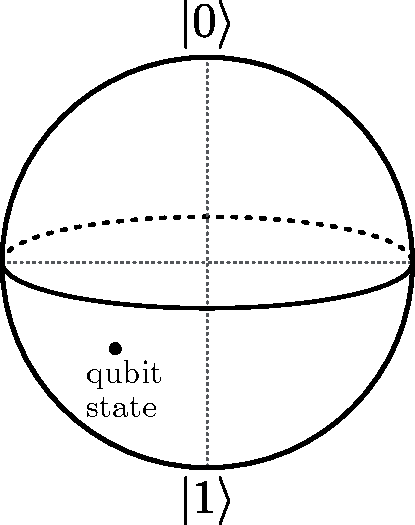
\includegraphics[width=0.3\linewidth]{bloch-sphere-1.pdf}} \hspace{10ex}
	\subfloat[]{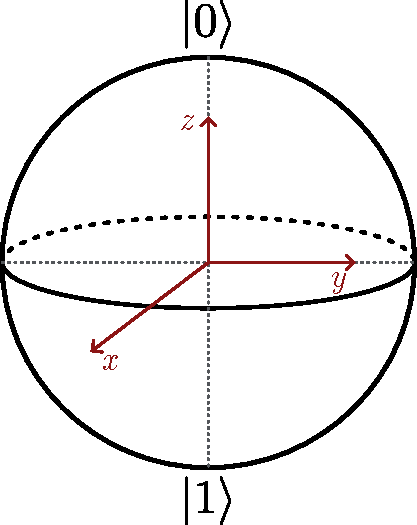
\includegraphics[width=0.3\linewidth]{bloch-sphere-2.pdf}}
	\caption{(a) Bloch sphere. (b) explicit $xyz$ coordinates.}
	\label{fig:bloch-sphere}
\end{figure}

As before, a single qubit can be represented by $\ket{\psi} = \alpha \ket{0} + \beta \ket{1}$, where $\abs{\alpha}^2 + \abs{\beta}^2 = 1$.
Note that although $\alpha$, $\beta$ can be imaginary, so it seems like we have four undetermined values, we only care about their relative phase.
So the most general representation for the state is in fact $\ket{\psi} = r_{\alpha} \ket{0} + r_{\beta} e^{i \phi} \ket{1}$.

If we apply the normalization criteria, we find:
\begin{align*}
	\braket{\psi}{\psi} &= 1 \\
	\ket{\psi} &= r_{\alpha} \ket{0} + (x + iy) \ket{1} \\
	\braket{\psi}{\psi} = r_{\alpha}^2 + x^2 + y^2 &= 1 \\
\end{align*}
which returns the equation for the unit sphere.

The usual parameterization for $\psi$ is $\ket{\psi} = \cos \frac{\theta}{2} \ket{0} + \sin \frac{\theta}{2} e^{i \phi} \ket{1}$.
This leads to the following convenient values:

\begin{align*}
	\theta = 0  &\rightarrow  \ket{0} \\
	\theta = \pi  &\rightarrow  \ket{1} \\
	\theta = \frac{\pi}{2}, \phi = 0  &\rightarrow  \ket{X} = \frac{1}{\sqrt{2}} \left( \ket{0} + \ket{1} \right) \\
	\theta = \frac{\pi}{2}, \phi = \frac{\pi}{2}  &\rightarrow  \ket{Y} = \frac{1}{\sqrt{2}} \left( \ket{0} + i\ket{1} \right) \\
\end{align*}

Logic gates represent motion on the surface.
For example, the \texttt{NOT} gate is given by $R(\pi)$ or rotation by $\pi = \SI{180}{\degree}$.

Another allowed quantum gate is the \textbf{Hadamard gate}, $H$, which maps

\begin{align*}
	\ket{0} &\rightarrow \frac{1}{\sqrt{2}} \left( \ket{0} + \ket{1} \right) = \ket{+} \\
	\ket{1} &\rightarrow \frac{1}{\sqrt{2}} \left( \ket{0} - \ket{1} \right) = \ket{-}
\end{align*}

In matrix representation, this is expressed as 

\[ H = \frac{1}{\sqrt{2}} \begin{pmatrix} 1 & 1 \\ 1 & -1 \end{pmatrix}\ \text{so}\ H \begin{pmatrix} 1 \\ 0 \end{pmatrix} = \begin{pmatrix} 1 & 1 \\ 1 & -1 \end{pmatrix} \begin{pmatrix} 1 \\ 0 \end{pmatrix} = \frac{1}{\sqrt{2}} \begin{pmatrix} 1 \\ 1 \end{pmatrix} \]

This generates equally weighted superposition states.
It is visualized as a rotation by $\pi/2$.

\section{2-qubit gates}

Consider the following setup:

\begin{figure}[!ht]
	\centering
	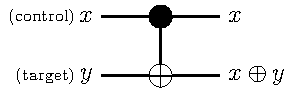
\includegraphics[height=0.8in]{cnot-1.pdf}
	\caption{CNOT gate}
	\label{fig:cnot-1}
\end{figure}

We'll now consider the \texttt{CNOT} operation (\autoref{fig:cnot-1}) which performs \texttt{NOT} on the second qubit only when the first qubit is 1.
That is, we have

\begin{align*}
	\ket{00} &\rightarrow \ket{00} \\
	\ket{01} &\rightarrow \ket{01} \\
	\ket{10} &\rightarrow \ket{11} \\
	\ket{11} &\rightarrow \ket{10} 
\end{align*}

In the matrix representation,

\[ U = \begin{pmatrix} 1 & 0 & 0 & 0 \\ 0 & 1 & 0 & 0 \\ 0 & 0 & 0 & 1 \\ 0 & 0 & 1 & 0 \end{pmatrix} \begin{pmatrix} 0 \\ 0 \\ 0 \\ 1 \end{pmatrix} = \begin{pmatrix} 0 \\ 0 \\ 1 \\ 0 \end{pmatrix} \]

\begin{figure}[!ht]
	\centering
	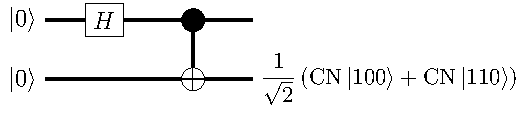
\includegraphics[height=0.8in]{cnot-2.pdf}
	\caption{Caption}
	\label{fig:cnot-2}
\end{figure}

\autoref{fig:cnot-2} has a simplified example of such a configuration.
On the control side, $\ket{0} \stackrel{H}{\rightarrow} \frac{1}{\sqrt{2}} \left( \ket{0} + \ket{1} \right)$.
For the target, $\ket{0} \rightarrow \frac{1}{\sqrt{2}} \left( \ket{00} + \ket{11} \right)$.
This is a maximally entangled state: If we measure qubit 1 ($Q_1$), we would get 0,1 with \SI{50}{\percent} probability.

Here's a thought experiment that reveals something interesting about this construction.
Suppose Alice takes $Q_1$ and Bob takes $Q_2$ and goes to Mars.
Now if Alice measures $Q_1$ to be $\ket{0}$, she instantly knows what Bob will measure, since the measurements are correlated.

But now suppose Alice first applies $H$ to her qubit, to get

\[ (H \otimes I) \frac{1}{\sqrt{2}} \left( \ket{00} + \ket{11} \right) = \frac{1}{2} \left( \ket{00} + \ket{10} + \ket{01} - \ket{11} \right) \]

Now if Alice measures $\ket{0}$, Bob's qubit collapses to $\frac{1}{\sqrt{2}} \left( \ket{0} + \ket{1} \right) = \ket{+}$.
But if Alice measures $\ket{1}$, Bob's qubit instantly goes to $\frac{1}{\sqrt{2}} \left( \ket{0} - \ket{1} \right) = \ket{-}$.
This is the signature of the famous EPR paradox.\footnote{Named after its formulators: Einstein, Podolsky, and Rosen, \href{https://link.aps.org/doi/10.1103/PhysRev.47.777}{\emph{Phys. Rev. Lett.}} 47, 1935.}

What is the quantum parallelism? 
Imagine we have a black box that takes input $x$ and outputs $f(x)$.
$x$ can take on values 0 and 1, as can $f(x)$.
We want to know if $f(0) = f(1)$ (constant) or $f(0) \neq f(1)$ (balanced).
Classically, we would need to measure both $f(0)$ and $f(1)$, but our box is so slow that each computation takes \SI{24}{\hour}. 
Instead, consider the following quantum gate (\texttt{CNOT}) in \autoref{fig:cnot-3}:

\begin{figure}[!ht]
	\centering
	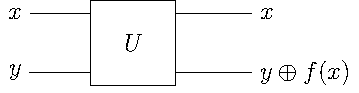
\includegraphics[width=0.4\linewidth]{cnot-3.pdf}
	\caption{Caption}
	\label{fig:cnot-3}
\end{figure}

where the $\oplus$ symbol represents addition modulo 2, and the result is that the second bit is flipped only if $f$ acting on the first qubit is 1 (otherwise does nothing).
Written out, this is 

\[ U: \ket{x,y} \rightarrow \ket{x, y \oplus f(x)} \]

To this machine we input the superposition state for the second qubit, $\frac{1}{\sqrt{2}}\left( \ket{0} - \ket{1} \right)$.
This would return:

\[ U: \ket{x, \frac{1}{\sqrt{2}} (\ket{0} - \ket{1})} \rightarrow \ket{x} \frac{1}{\sqrt{2}} (\ket{f(x)} - \ket{1 \oplus f(x)}) = \ket{x} (-1)^{f(x)} \frac{1}{\sqrt{2}} ( \ket{0} - \ket{1} )\]

and so $f$ determines the phase of the output! 

OK, so now let's consider making the first qubit also a superposition:

\begin{align*}
	U: \ket{\frac{1}{\sqrt{2}} (\ket{0} - \ket{1}), \frac{1}{\sqrt{2}} (\ket{0} - \ket{1})} &\rightarrow 
	\frac{1}{2} \left( U \ket{0} (\ket{0} - \ket{1}) + U \ket{1} (\ket{0} - \ket{1}) \right) \\
	&= \frac{1}{2} \left[ (-1)^{f(0)} \ket{0} + (-1)^{f(1)} \ket{1} \right]  (\ket{0} - \ket{1}) \\
\end{align*}

\begin{figure}[!ht]
	\centering
	\subfloat[]{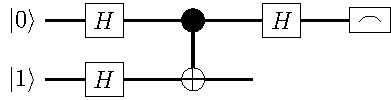
\includegraphics[height=0.7in]{epr-1.pdf}} \hspace{10ex}
	\subfloat[]{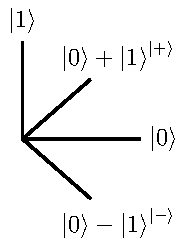
\includegraphics[height=1.8in]{epr-2.pdf}}
	\caption{EPR paradox}
	\label{fig:epr}
\end{figure}

We illustrate this in \autoref{fig:epr}.
Now we apply the Hadamard operator on the first qubit:

\begin{align*}
	H \left[ (-1)^{f(0)} \ket{0} + (-1)^{f(1)} \ket{1} \right] &\rightarrow
	(-1)^{f(0)} (\ket{0} + \ket{1}) + (-1)^{f(1)} (\ket{0} - \ket{1}) \\
	&= \left( (-1)^{f(0)} + (-1)^{f(1)} \right) \ket{0} + \left( (-1)^{f(0)} - (-1)^{f(1)} \right) \ket{1}
\end{align*}

And now we try to make a measurement in the $\ket{0}$, $\ket{1}$ basis. 
If $f(0) = f(1)$ (constant), then we always measure $\ket{0}$ with a \SI{100}{\percent} probability.
On the other hand, if $f(0) \neq f(1)$ (balanced), then we always measure $\ket{1}$.
This is the quantum parallelism, and it shows how one can manipulate states to determine measurement outcomes. 

\section{Quantum teleportation}

Now let's see how we can take advantage of entanglement. 
We'll start with a EPR pair: $\frac{1}{\sqrt{2}} (\ket{00} + \ket{11})$.
Recall we can generate this using the protocol in \autoref{fig:cnot-2}.
Alice takes the first qubit, while Bob takes the 2nd one and travels.
Now Alice wants to deliver a qubit $\ket{\psi}$ to Bob, where $\ket{\psi} = \alpha \ket{0} + \beta \ket{1}$.
Note the following:

\begin{itemize}
	\item Alice doesn't know the state of the qubit she wants to send!
	
	\item If she measured it, she would just measure one state, which is not enough to reconstruct the wavefunction.
	
	\item Even if she did know $\ket{\psi}$, it would take infinite information to send! 
	(recall $\alpha$ and $\beta$ are continuous)
	
	\item Yet we will show she can teleport quantum state with 2 bits of information!
	
	\item If an observer intercepts the qubit, the information is useless.
	We need the second qubit as a key to decode.
	Thus Alice doesn't need to know where Bob is! 
	She just has to broadcast the information.
\end{itemize}

\begin{figure}[!ht]
	\centering
	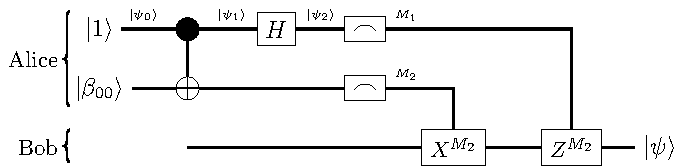
\includegraphics[width=\linewidth]{three-qubit.pdf}
	\caption{Three-qubit problem.}
	\label{fig:three-qubit}
\end{figure}

\autoref{fig:three-qubit} presents the 3-qubit problem, where Alice has two of them.
The input ``s a $\ket{\psi_o}$" equals

\[ \ket{\psi} \ket{\beta_{00}} = \left( \alpha \ket{0} + \beta \ket{1} \right) \otimes \frac{1}{\sqrt{2}} \left( \ket{00} + \ket{11} \right) = \frac{1}{\sqrt{2}} \left( \alpha \ket{000} + \alpha \ket{011} + \beta \ket{100} + \beta \ket{111} \right) \]

After \texttt{CNOT}, $\ket{\psi_1} = \frac{1}{\sqrt{2}} \left( \alpha \ket{000} + \alpha \ket{011} + \beta \ket{110} + \beta \ket{101} \right)$.

After $H$, $\ket{\psi_2} = \frac{1}{2} \left( \alpha \ket{000} + \alpha \ket{100} + \alpha \ket{011} + \alpha \ket{111} + \beta \ket{01} - \beta \ket{110} + \beta \ket{001} - \beta \ket{101} \right)$.

Now Alice measures her qubit and send the result to Bob.
The outcomes are summarized in \autoref{tab:three-qubit}.

\begin{table}[!ht]
	\centering
	\begin{tabular}{cc}
		If Alice sees: & Then Bob's qubit is: \\
		\toprule 
		$\ket{00}$ & $\alpha \ket{0} + \beta \ket{1}$ \\
		$\ket{1}$ $\ket{10}$ & $\alpha \ket{1}$ $\beta \ket{0}$ $\alpha \ket{0} - \beta \ket{1}$ \\
		$\ket{11}$ & $\alpha \ket{1} - \beta \ket{0}$
	\end{tabular}
	\caption{Caption}
	\label{tab:three-qubit}
\end{table}

Teleportation is complete if $\ket{00}$ is measured.
If $\ket{01}$ is measured, Bob just applies $X$ gate.
If $\ket{10}$ is measured, apply $Z$ gate.
If $\ket{11}$ is measured, apply both $X$ and $Z$.

\section[General comments]{General comments on entanglement}

For a single spin, the basis is $\ket{\uparrow}$ and $\ket{\downarrow}$.
A superposition state is composed of $c_{\uparrow} \ket{\uparrow} + c_{\downarrow} \ket{\downarrow}$.

For two spins, the basis is $\ket{\uparrow} \ket{\uparrow}$, $\ket{\uparrow} \ket{\downarrow}$, $\ket{\downarrow} \ket{\uparrow}$, and $\ket{\downarrow} \ket{\downarrow}$.
In this case, the general superposition state would be $a \ket{\uparrow \uparrow} + b \ket{\uparrow \downarrow} + c \ket{\downarrow \uparrow} + d \ket{\downarrow \downarrow}$.

The Key point: This general superposition state of two qubits cannot generally be written as the product $\left( c_{\uparrow}^1 \ket{\uparrow} + c_{\downarrow}^1 \ket{\downarrow} \right) \left( c_{\uparrow}^2 \ket{\uparrow} + c_{\downarrow}^2 \ket{\downarrow} \right)$.
In other words, one cannot say spin 1 is in one state and spin 2 is in another.
Rather, they are \textbf{entangled}.

For example, the product $\ket{\uparrow} \ket{\downarrow}$ is \emph{entangled}.
This is because $\ket{\uparrow \downarrow} + \ket{\downarrow \downarrow} = \left( \ket{\uparrow} + \ket{\downarrow} \right) \ket{\downarrow}$ is not entangled.
Here, the second spin is definitely down.

But $\ket{\uparrow \uparrow} + \ket{\downarrow \downarrow}$ or $\ket{\uparrow \downarrow} - \ket{\downarrow \uparrow}$ are. 
We can't say what state spin 1 is in.
A measurement gives up or down with \SI{50}{\percent} probability, but there are hidden correlations.

Black hole entanglement: Ads/LET: Linkage between entanglement and gravity.

ER : EPR : Wormhole = 2 entangled black holes.

Can we test quantum gravity in the laboratory via the creation of entangled states?


%%%%%%%%%%%%%%%%%%%%%%%%%%%%%%%%%%%%%%%%%%%%%%%%%%%%%%%%%%%%%%%%%%%%%%%%%%%%%%%%

\section[Applications]{Application: Superconducting qubits or spin qubits in Si}

Superconducting Qubits: Superconducting materials are among the most widely used implementations of qubits. You can explore how materials such as niobium and aluminum are employed to create Josephson junctions, essential for superconducting qubits. Discuss the quantum coherence of these materials and how their superconducting properties enable low-resistance pathways, crucial for creating stable qubit states that elevate the performance of quantum processors.

Spin Qubits in Silicon: Highlight how silicon, a well-known semiconductor, is being explored for encoding qubits using the spin of electrons or nuclei. You can cover topics on how impurities in silicon can be utilized to create qubit systems and the ongoing research to integrate quantum computing with classical silicon-based technology. Discussing the material's advantages (like the existing fabrication infrastructure from classical computing) could also resonate well with students.

N-V centers in diamond?


%%%%%%%%%%%%%%%%%%%%%%%%%%%%%%%%%%%%%%%%%%%%%%%%%%%%%%%%%%%%%%%%%%%%%%%%%%%%%%%%

\section{Summary}
To recap, in this chapter we analyzed...

%} % for doublespacing
\end{document}